%
% DS 5110 (Blue Team) Project Proposal
%
\documentclass[12pt]{article}

%
% Packages
%
\usepackage{amsmath}
\usepackage{enumerate}
\usepackage[utf8]{inputenc}

\RequirePackage{graphics}

\usepackage{graphicx}
\graphicspath{ {imgs/} }

%
% Document Settings
%
\setlength{\parskip}{1pc}
\setlength{\parindent}{0pt}
\setlength{\topmargin}{-3pc}
\setlength{\textheight}{9.5in}
\setlength{\oddsidemargin}{0pc}
\setlength{\evensidemargin}{0pc}
\setlength{\textwidth}{6.5in}

\title{DS 5110: Project - Fall 2017}
\author{Tyler Brown, Sicheng Hao, Nischal Mahaveer Chand, Sumedh Sankhe}
\date{ }


% START DOCUMENT
\begin{document}

\maketitle

\section*{Summary}

When we put ourselves in the shoes of potential homebuyers in the
Greater Boston area, we find that they have many informational resources
available. As a homebuyer, their major sources of information are the
websites Zillow \cite{ZillowRe12:online} and Trulia
\cite{TruliaRe98:online}. These resources provide information such as
home location, price, amenties, and types. Trulia differentiates itself
by providing a ``Local Scoop'', giving the homebuyer maps of crime, school
location, and the relative distribution of home prices in Greater
Boston. However, neither of these websites provide information about how
neighborhoods are changing over time.

Homebuyers want to better understand their potentially new communities.
It's helpful to know if your neighbors have been regularly developing
and maintaining their properties. A homebuyer would also like to know
whether a neighborhood as been experiencing various levels of turnover.
The problem our group is focusing on is how we can help these new
homebuyers by presenting them with an inuitive way to understand how
their potential neighborhoods have been changing over time.

The City of Boston provides an open data platform, Analyze Boston, 
containing information related to our lives in the city. Property 
assessment data from 2014-2017 is one of the resources available on their
 open data platform. Included in the property assessment data is 
``property, or parcel, ownership together with information about value, 
which ensures fair assessment of Boston taxable and non-taxable property 
of all types and classifications'' \cite{Property49:online}. Our team 
has aggregated each available year to create a time series dataset of 
Property Assessments in Boston. This aggregated dataset allows us to 
provide unique insights into property valuations and ownership strategies.

\section*{Proposed Plan of Research}

The datasets we are having right now are separate yearly. The first step 
we are going to do is merge them into one single file. Then we are going 
to do some necessary cleaning for the data set. 

In the second step, we are going to filter out the data that could 
represent the problem we are trying to solve. Maybe add some data from 
other sources( like Google Maps or Zillow)

To help people understand the data better. In the last step we will make 
an interactive Shiny application to visualize our finding. 


\section*{Preliminary Results}

Our preliminary results include a data audit and descriptive findings.
The data audit found trouble spots in our data such as missing values or
incomplete values for coordinates as well as a small number of duplicate
values for the given primary keys. The descriptive findings generated
possible directions for our research question such as changes in 
property valuations, dominant ownership strategies for owners 
controlling a higher percentage of Boston property, and changes in
property valuations for various land usage types.

\subsection*{Data Audit Findings}

The major data audit findings are (1) the given primary keys, $PID$, are 
not unique for 0.3\% because they are mapped to multiple geographic 
coordinate pairs, (2) about 22\% of geographic coordinates are either 
missing or unusable, (3) about 10\% of property parcels, identified with
$PID$ do not pay taxes. Of that 10\%, we can explain about 49\% of this 
variation due to tax-exempt land use status. The remaining 51\% is 
associated with the "Condominium main" land usage type. It's unclear why 
there are zero taxes associated with this land usage type without 
contacting the city of Boston. This anomaly effects about 5\% of the 
total data.

\subsection*{Descriptive Findings}
Preliminary relationships found within the data are (1) residential 
condominium units appear to have the lowest proportion of value but 
previously we saw they had the second-highest proportion of gross tax,
(2) residential family and residential land appears to have gained the 
most value from 2014-2017, (3) the most significant gains in property
assessment from 2014-2017 have been made land used for commerical and
commerical condominium properties, (4) those who are further away from 
the financial district appear to be generally paying a lower proportion 
of taxes, and (5) larger real estate developers appear to choose one
of two distinct strategies that involve either paying higher taxes with
less property or lower taxes with more property. The figure below shows
how location might effect changes in property assessments from 2014-2017.

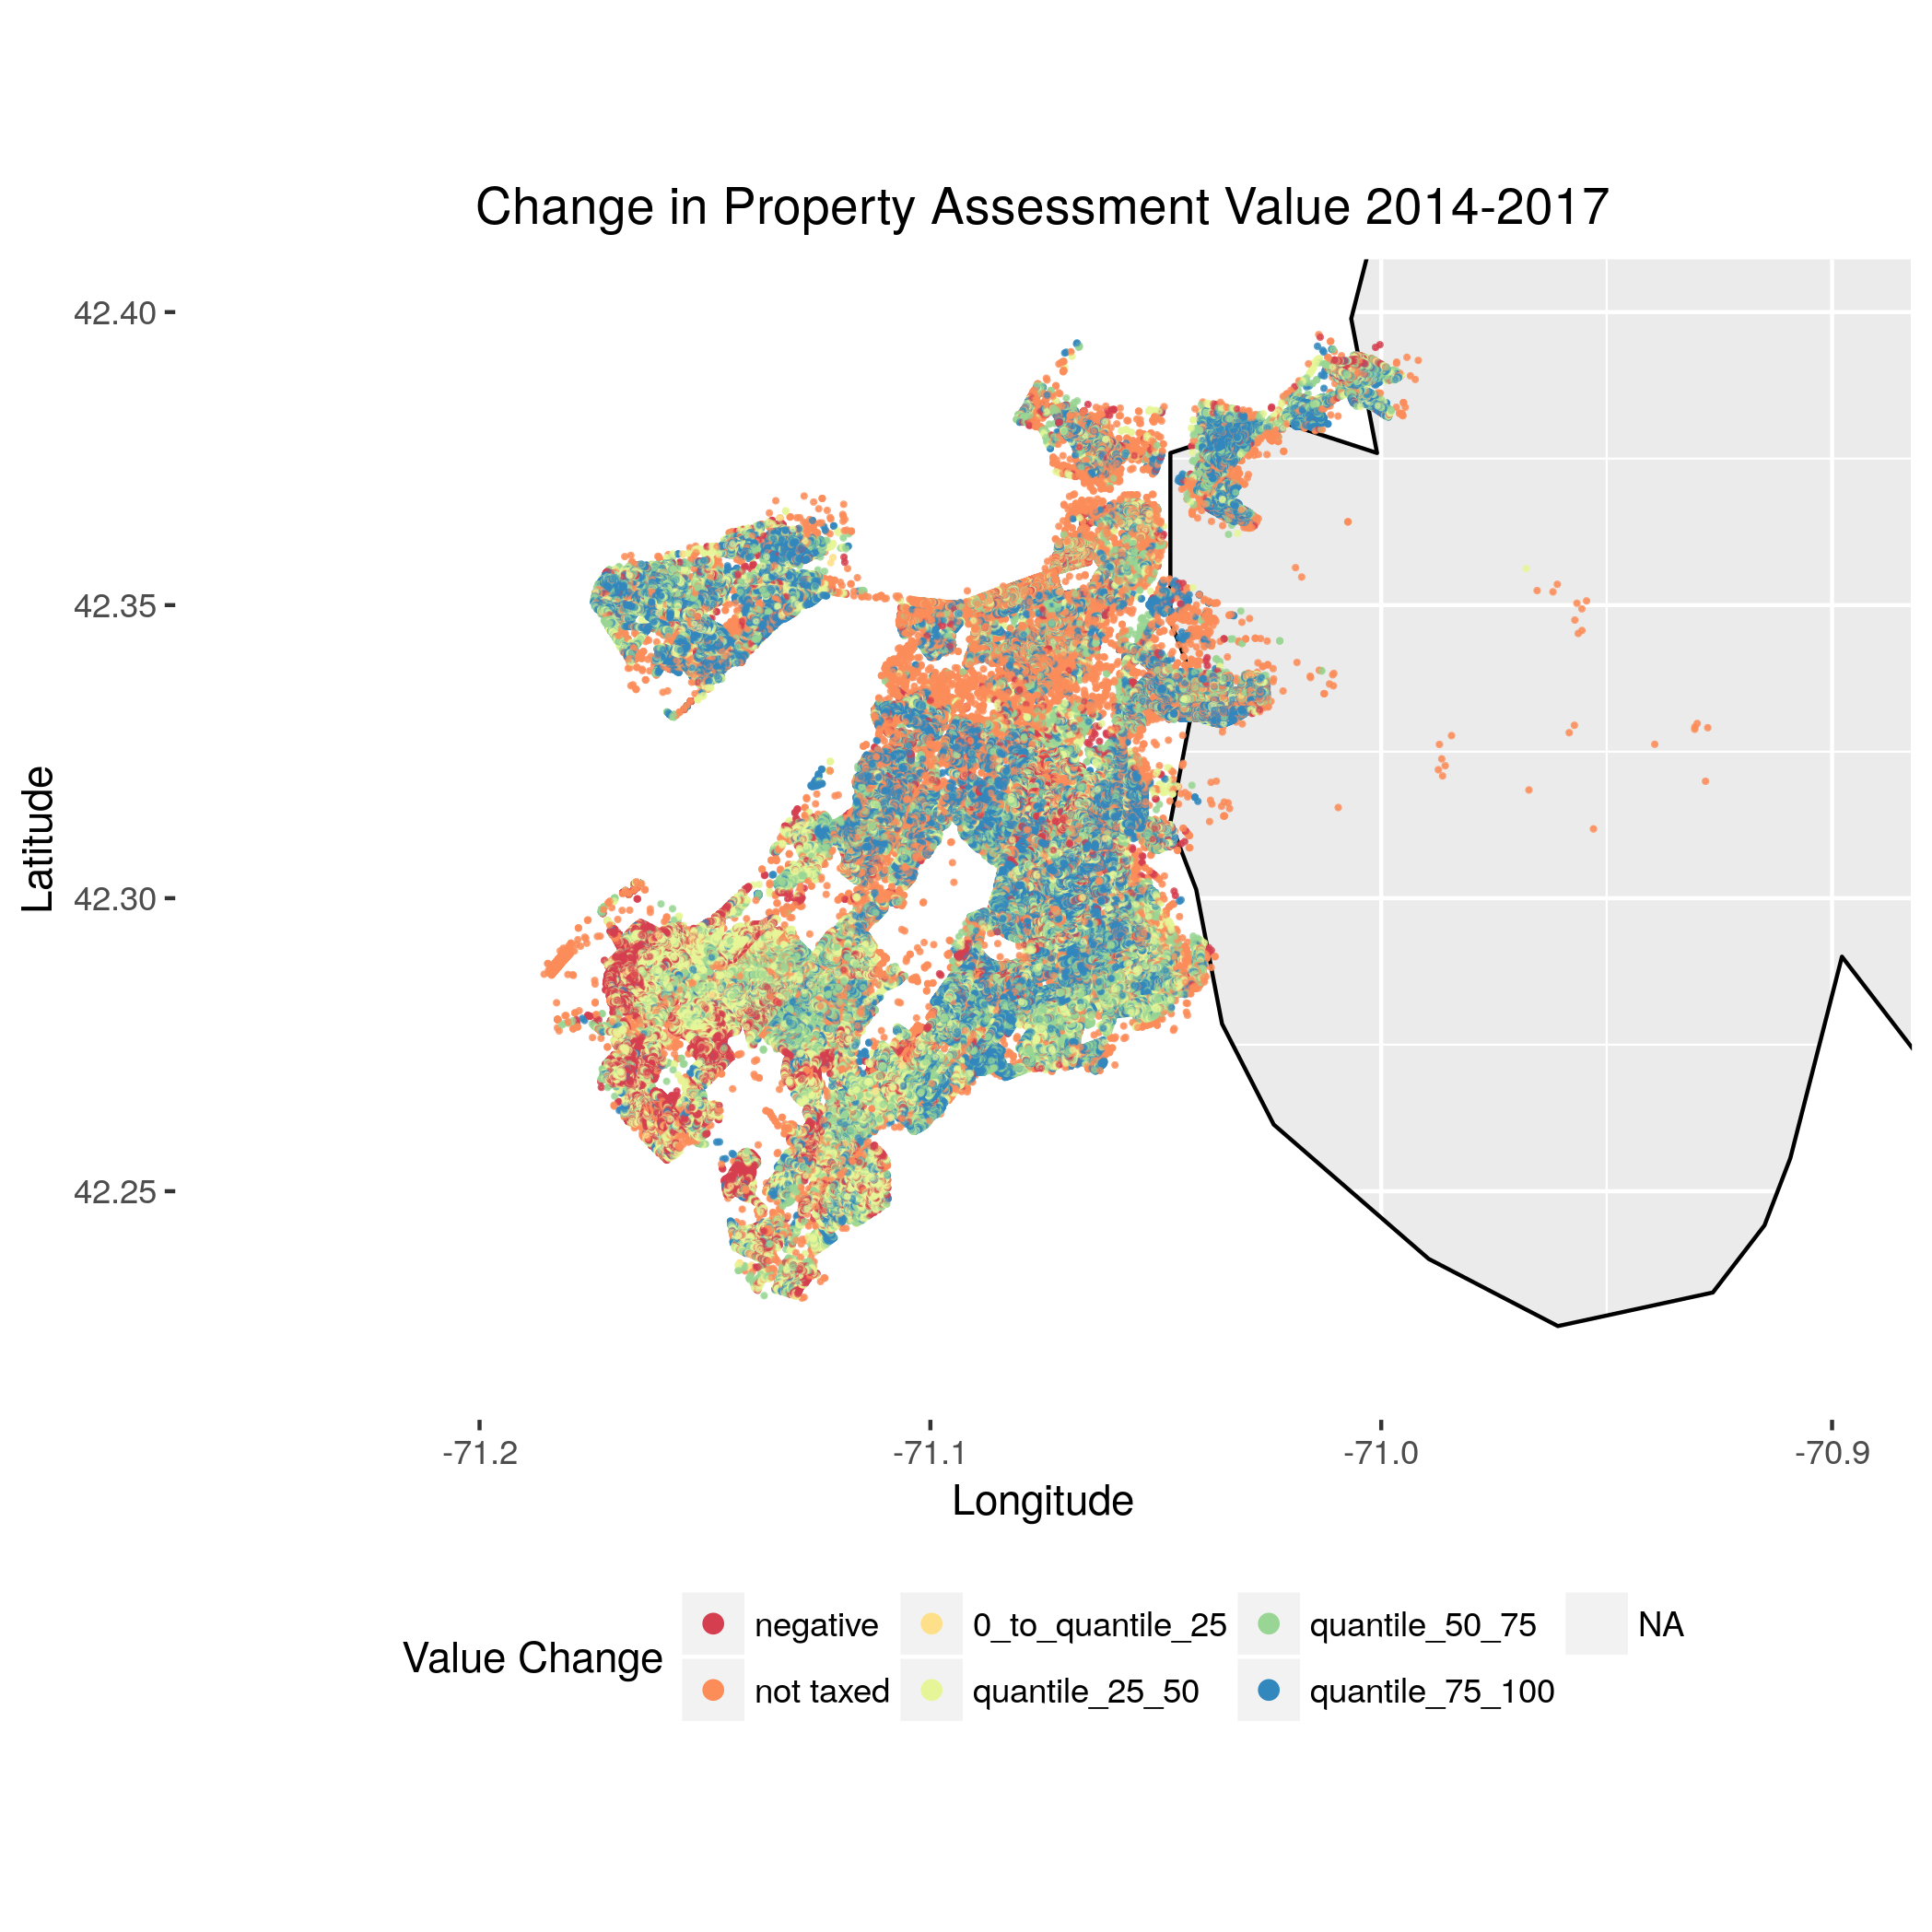
\includegraphics[scale=0.75]{property_delta2014-2017}


\bibliography{references} 
\bibliographystyle{ieeetr}

\end{document}
